\documentclass[11pt,a4paper]{article}

% ========== PACKAGES ==========
\usepackage[utf8]{inputenc}
\usepackage[T1]{fontenc}
\usepackage{lmodern}
\usepackage{textcomp}
\usepackage{arevtext}
\usepackage[margin=1in]{geometry}
\usepackage{graphicx}
\usepackage{xcolor}
\usepackage{titlesec}
\usepackage{enumitem}
\usepackage{hyperref}
\usepackage{fancyhdr}
\usepackage{tabularx}
\usepackage{booktabs}
\usepackage{fontawesome5}
\usepackage{tcolorbox}
\usepackage{tikz}
\usepackage{pifont}
\newcommand{\rupee}{\text{\textrupee}}
\usepackage{setspace}
\usepackage{multicol}
\usepackage{colortbl}

\tcbuselibrary{skins,breakable}

% ========== COLORS ==========
\definecolor{primary}{RGB}{16, 185, 129}      % Emerald Green
\definecolor{secondary}{RGB}{10, 10, 10}      % Pure Black
\definecolor{accent}{RGB}{239, 68, 68}        % Red
\definecolor{darkbg}{RGB}{13, 13, 13}
\definecolor{textgray}{RGB}{156, 163, 175}
\definecolor{headerblue}{RGB}{41, 65, 114}
\definecolor{lightblue}{RGB}{230, 236, 245}
\definecolor{lightgreen}{RGB}{230, 245, 235}
\definecolor{warnyellow}{RGB}{251, 191, 36}
\definecolor{purpleaccent}{RGB}{139, 92, 246}

% ========== STYLING ==========
\hypersetup{
    colorlinks=true,
    linkcolor=primary,
    urlcolor=primary,
    pdfauthor={Priyanshu},
    pdftitle={iStocks - AI-Native Investment Platform for Bharat}
}

\titleformat{\section}{\Large\bfseries\color{primary}}{}{0em}{}
\titleformat{\subsection}{\large\bfseries\color{black}}{}{0em}{}
\titleformat{\subsubsection}{\normalsize\bfseries\color{textgray}}{}{0em}{}

\pagestyle{fancy}
\fancyhf{}
\fancyhead[L]{\textcolor{textgray}{\small iStocks | AI-Native Thesis Pitch}}
\fancyhead[R]{\textcolor{textgray}{\small \thepage}}
\renewcommand{\headrulewidth}{0.5pt}
\renewcommand{\headrule}{\hbox to\headwidth{\color{primary}\leaders\hrule height \headrulewidth\hfill}}

\setlength{\parindent}{0pt}
\setlength{\parskip}{8pt}

% ========== CUSTOM BOXES ==========
\newtcolorbox{featurebox}[1][]{
    colback=primary!5,
    colframe=primary,
    fonttitle=\bfseries,
    title=#1,
    rounded corners,
    boxrule=1pt,
    left=8pt, right=8pt, top=6pt, bottom=6pt
}

\newtcolorbox{highlightbox}[1][]{
    colback=primary!5,
    colframe=primary!60,
    fonttitle=\bfseries,
    title=#1,
    rounded corners,
    boxrule=0.8pt,
    left=8pt, right=8pt, top=6pt, bottom=6pt
}

\newtcolorbox{riskbox}[1][]{
    colback=accent!5,
    colframe=accent!60,
    fonttitle=\bfseries,
    title=#1,
    rounded corners,
    boxrule=0.8pt,
    left=8pt, right=8pt, top=6pt, bottom=6pt
}

\newtcolorbox{fixbox}[1][]{
    colback=primary!5,
    colframe=primary!60,
    rounded corners,
    boxrule=0.5pt,
    left=6pt, right=6pt, top=4pt, bottom=4pt
}

\newtcolorbox{purplebox}[1][]{
    colback=purpleaccent!5,
    colframe=purpleaccent!60,
    fonttitle=\bfseries,
    title=#1,
    rounded corners,
    boxrule=0.8pt,
    left=8pt, right=8pt, top=6pt, bottom=6pt
}

\newtcolorbox{statbox}{
    colback=lightgreen,
    colframe=primary!40,
    rounded corners,
    boxrule=0.5pt,
    left=12pt, right=12pt, top=8pt, bottom=8pt
}

% ========== DOCUMENT ==========
\begin{document}

% ========== TITLE PAGE ==========
\begin{titlepage}
    \centering
    \vspace*{2cm}
    
    % Logo
    
\begin{tikzpicture}
        \fill[primary, rounded corners=8pt] (0,0) rectangle (2,2);
        \draw[white, ultra thick, ->, >=stealth] (0.3,0.5) -- (1,1.5) -- (1.7,0.8);
    \end{tikzpicture}
    
    \vspace{1cm}
    
    {\Huge\bfseries\textcolor{primary}{iStocks}}\\[0.5cm]
    {\Large\textcolor{textgray}{AI-Native Investment Platform for Bharat}}
    
    \vspace{1.5cm}
    
    \rule{0.6\textwidth}{1pt}
    
    \vspace{1.5cm}
    
    {\large\textbf{Thesis Pitch Deck}}\\[0.3cm]
    {\normalsize Theme: AI $\times$ Investments for Bharat}
    
    \vspace{2cm}
    
    \begin{tcolorbox}[
        colback=primary!5,
        colframe=primary,
        width=0.75\textwidth,
        rounded corners,
        boxrule=1pt
    ]
    \centering
    {\normalsize Empowering \textbf{100M+ Indians} to invest smarter \\with conversational AI, real-time analytics, \\and algo-trading \textbf{in their own language}.}
    \end{tcolorbox}
    
    \vspace{2cm}
    
    {\normalsize\textcolor{textgray}{Live at: \textcolor{primary}{\url{https://istocks.codes}}}}\\[0.3cm]
    {\normalsize\textcolor{textgray}{\faAndroid~Android APK | Coming soon to Play Store}}
    
    \vfill
    
    {\small\textcolor{textgray}{April 2026}}\\[0.3cm]
    {\normalsize\textbf{Created by: Priyanshu}}
    
\end{titlepage}

% ========== TABLE OF CONTENTS ==========
\tableofcontents
\newpage


%==============================================================================
% 1. WHAT IS THE PRODUCT?
%==============================================================================
\section{What is iStocks?}

\textbf{iStocks} is India's first \textbf{AI-native trading intelligence platform} powered by an expert system of AI agents. It enables retail investors to analyze stocks, build trading strategies, and make informed investment decisions using \textbf{natural language}, in English and all Indian regional languages.

\begin{featurebox}[Core Value Proposition]
\textit{``Ask a question in plain Hindi. Get institutional-grade analysis. Build and deploy algo strategies. No coding. No jargon. Just intelligent investing.''}
\end{featurebox}

\subsection{Key Features}

\begin{tabularx}{\textwidth}{>{\bfseries}p{4cm}X}
\toprule
\textbf{Feature} & \textbf{Description} \\
\midrule
\faRobot~AI Stock Analyst & Powered by \textbf{Angle 3.0}, a collection of expert AI agents. Ask ``How is Reliance performing?'' and receive detailed technical + fundamental analysis with actionable insights. \\
\addlinespace
\faChartLine~40+ Technical Indicators & RSI, MACD, Bollinger Bands, EMA, SMA, ADX, OBV, Stochastic Oscillator, ATR, CCI, Williams \%R, ROC, and more, computed in real-time on live NSE/BSE data. \\
\addlinespace
\faFlask~Sangraha (Strategy Repo) & ``Sangraha'' (Sanskrit for collection), a community-driven strategy repository. Create, backtest, fork \& share trading strategies. A GitHub for algo trading. \\
\addlinespace
\faChartBar~Trading Agent & Intelligent trading agent that can analyze market conditions, identify entry/exit points, and execute trades automatically based on your strategy parameters. \\
\addlinespace
\faGlobe~Regional Language NLP & Full support for Hindi, Tamil, Telugu, Marathi, Bengali, and all Indian languages. First trading platform to truly serve \textit{Bharat}. \\
\addlinespace
\faMobile~Web + Android & Live at \url{istocks.codes} and as an Android APK. Will soon be deployed on Google Play Store. \\
\bottomrule
\end{tabularx}

\subsection{How Angle 3.0 Works}

\textbf{Angle 3.0} is our proprietary collection of specialized AI agents that work together to deliver institutional-grade analysis:

\begin{itemize}[leftmargin=*]
    \item \textbf{Analysis Agent:} Processes 40+ technical indicators and identifies patterns, trends, and signals in real-time.
    \item \textbf{Strategy Agent:} Builds, backtests, and optimizes trading strategies based on user preferences.
    \item \textbf{Trading Agent:} Monitors markets and executes trades automatically at optimal entry/exit points.
    \item \textbf{Language Agent:} Translates all interactions into the user's preferred Indian language seamlessly.
    \item \textbf{Risk Agent:} Evaluates portfolio risk, sets stop-losses, and protects users from emotional trading.
\end{itemize}

\subsection{Live Product Screenshots}

\textbf{Real-Time Stock Dashboard:}

\begin{center}
    \fbox{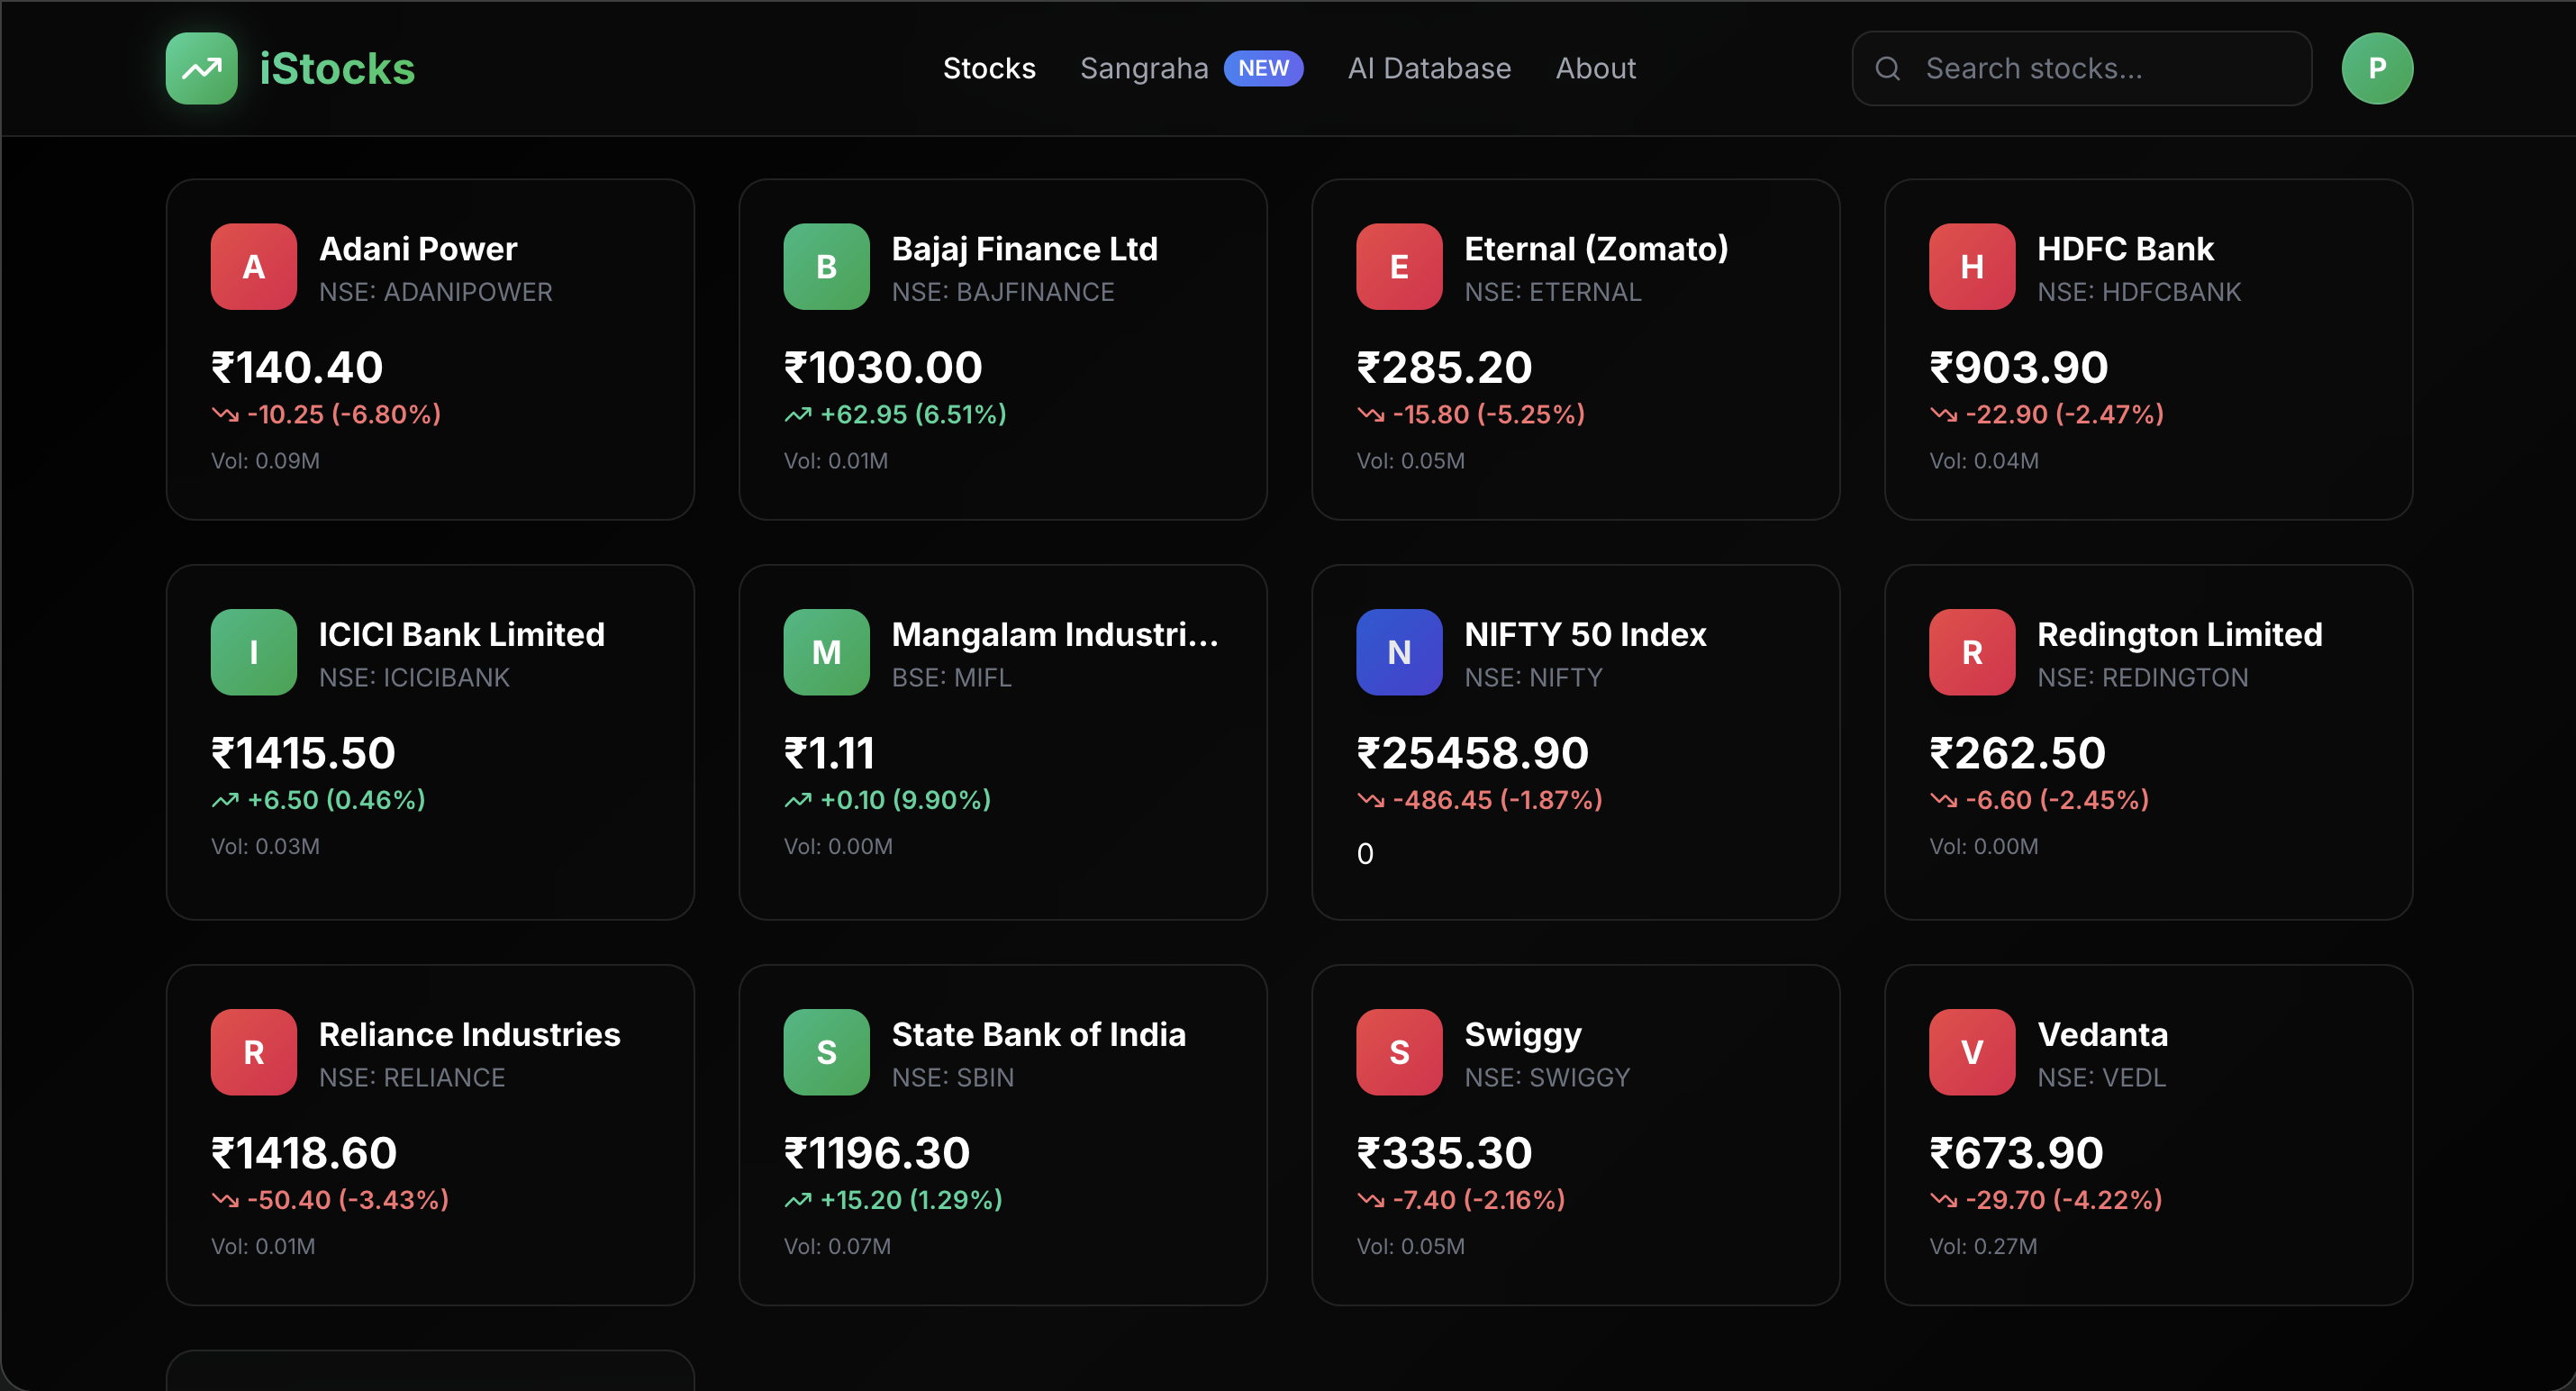
\includegraphics[width=0.95\textwidth]{Dashboard.png}}
\end{center}

\textbf{AI Stock Analyst, Conversational Analysis:}

\begin{center}
    \fbox{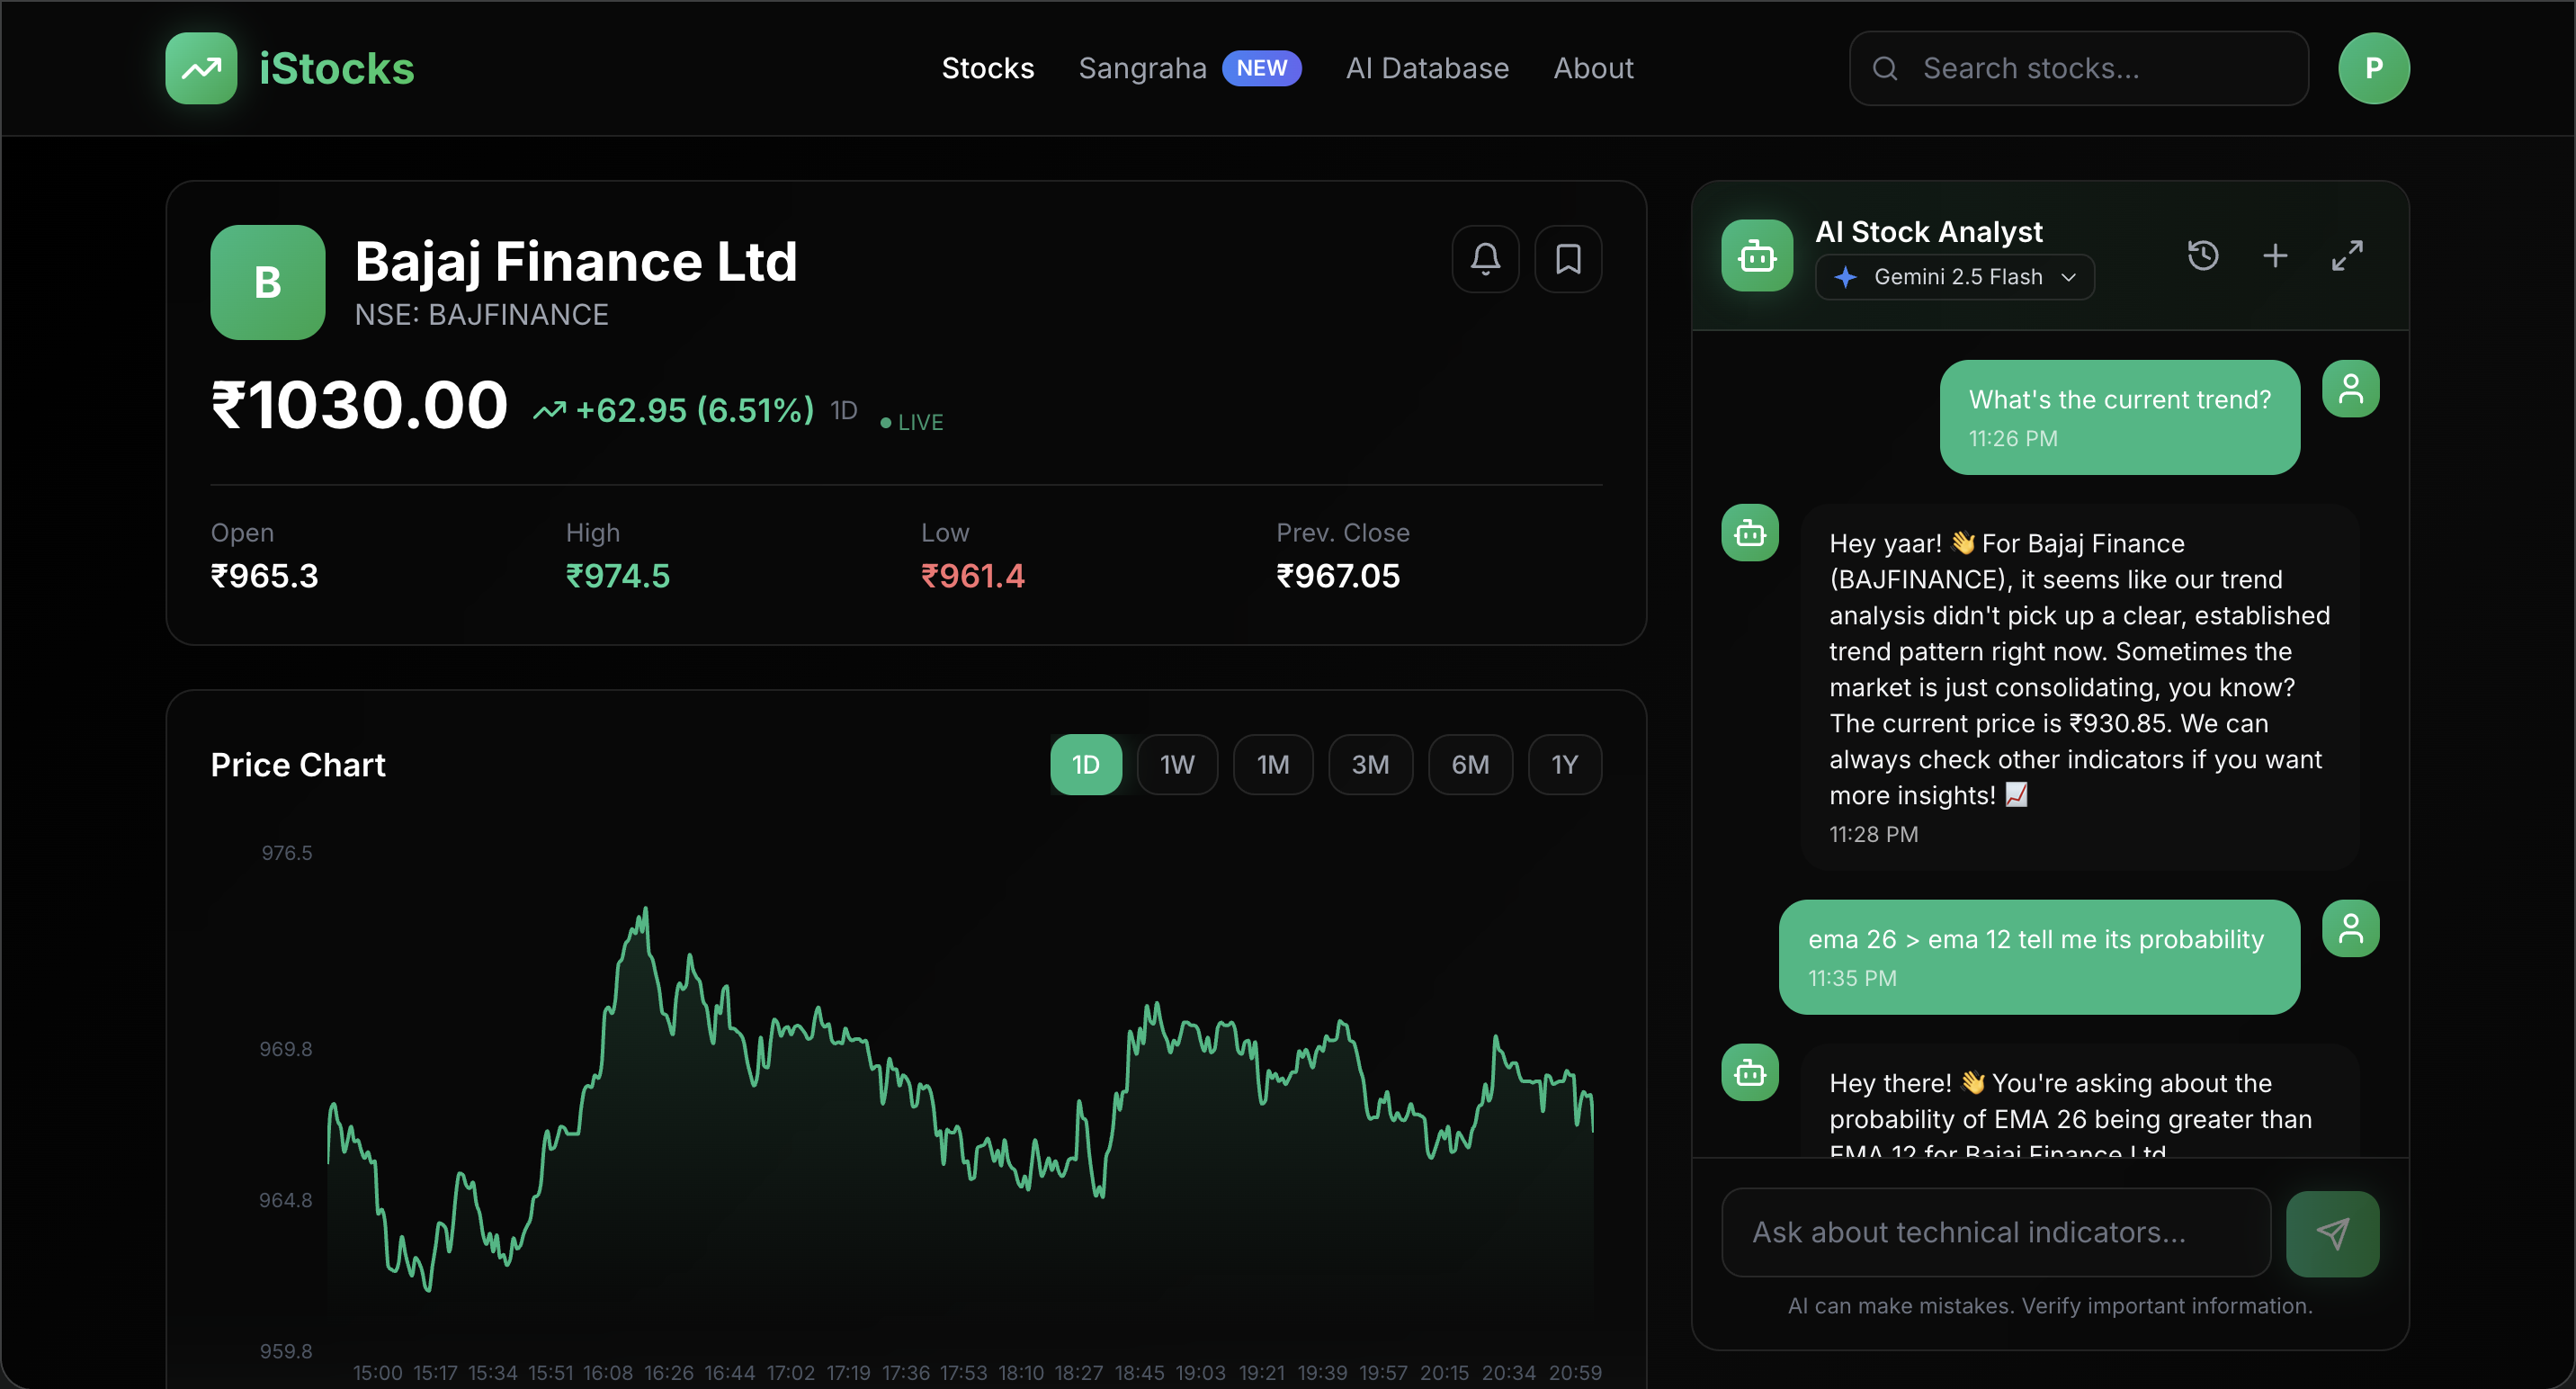
\includegraphics[width=0.95\textwidth]{Stock_analysis.png}}
\end{center}

\textbf{Trading Agent, Intelligent Trade Execution:}

\begin{center}
    \fbox{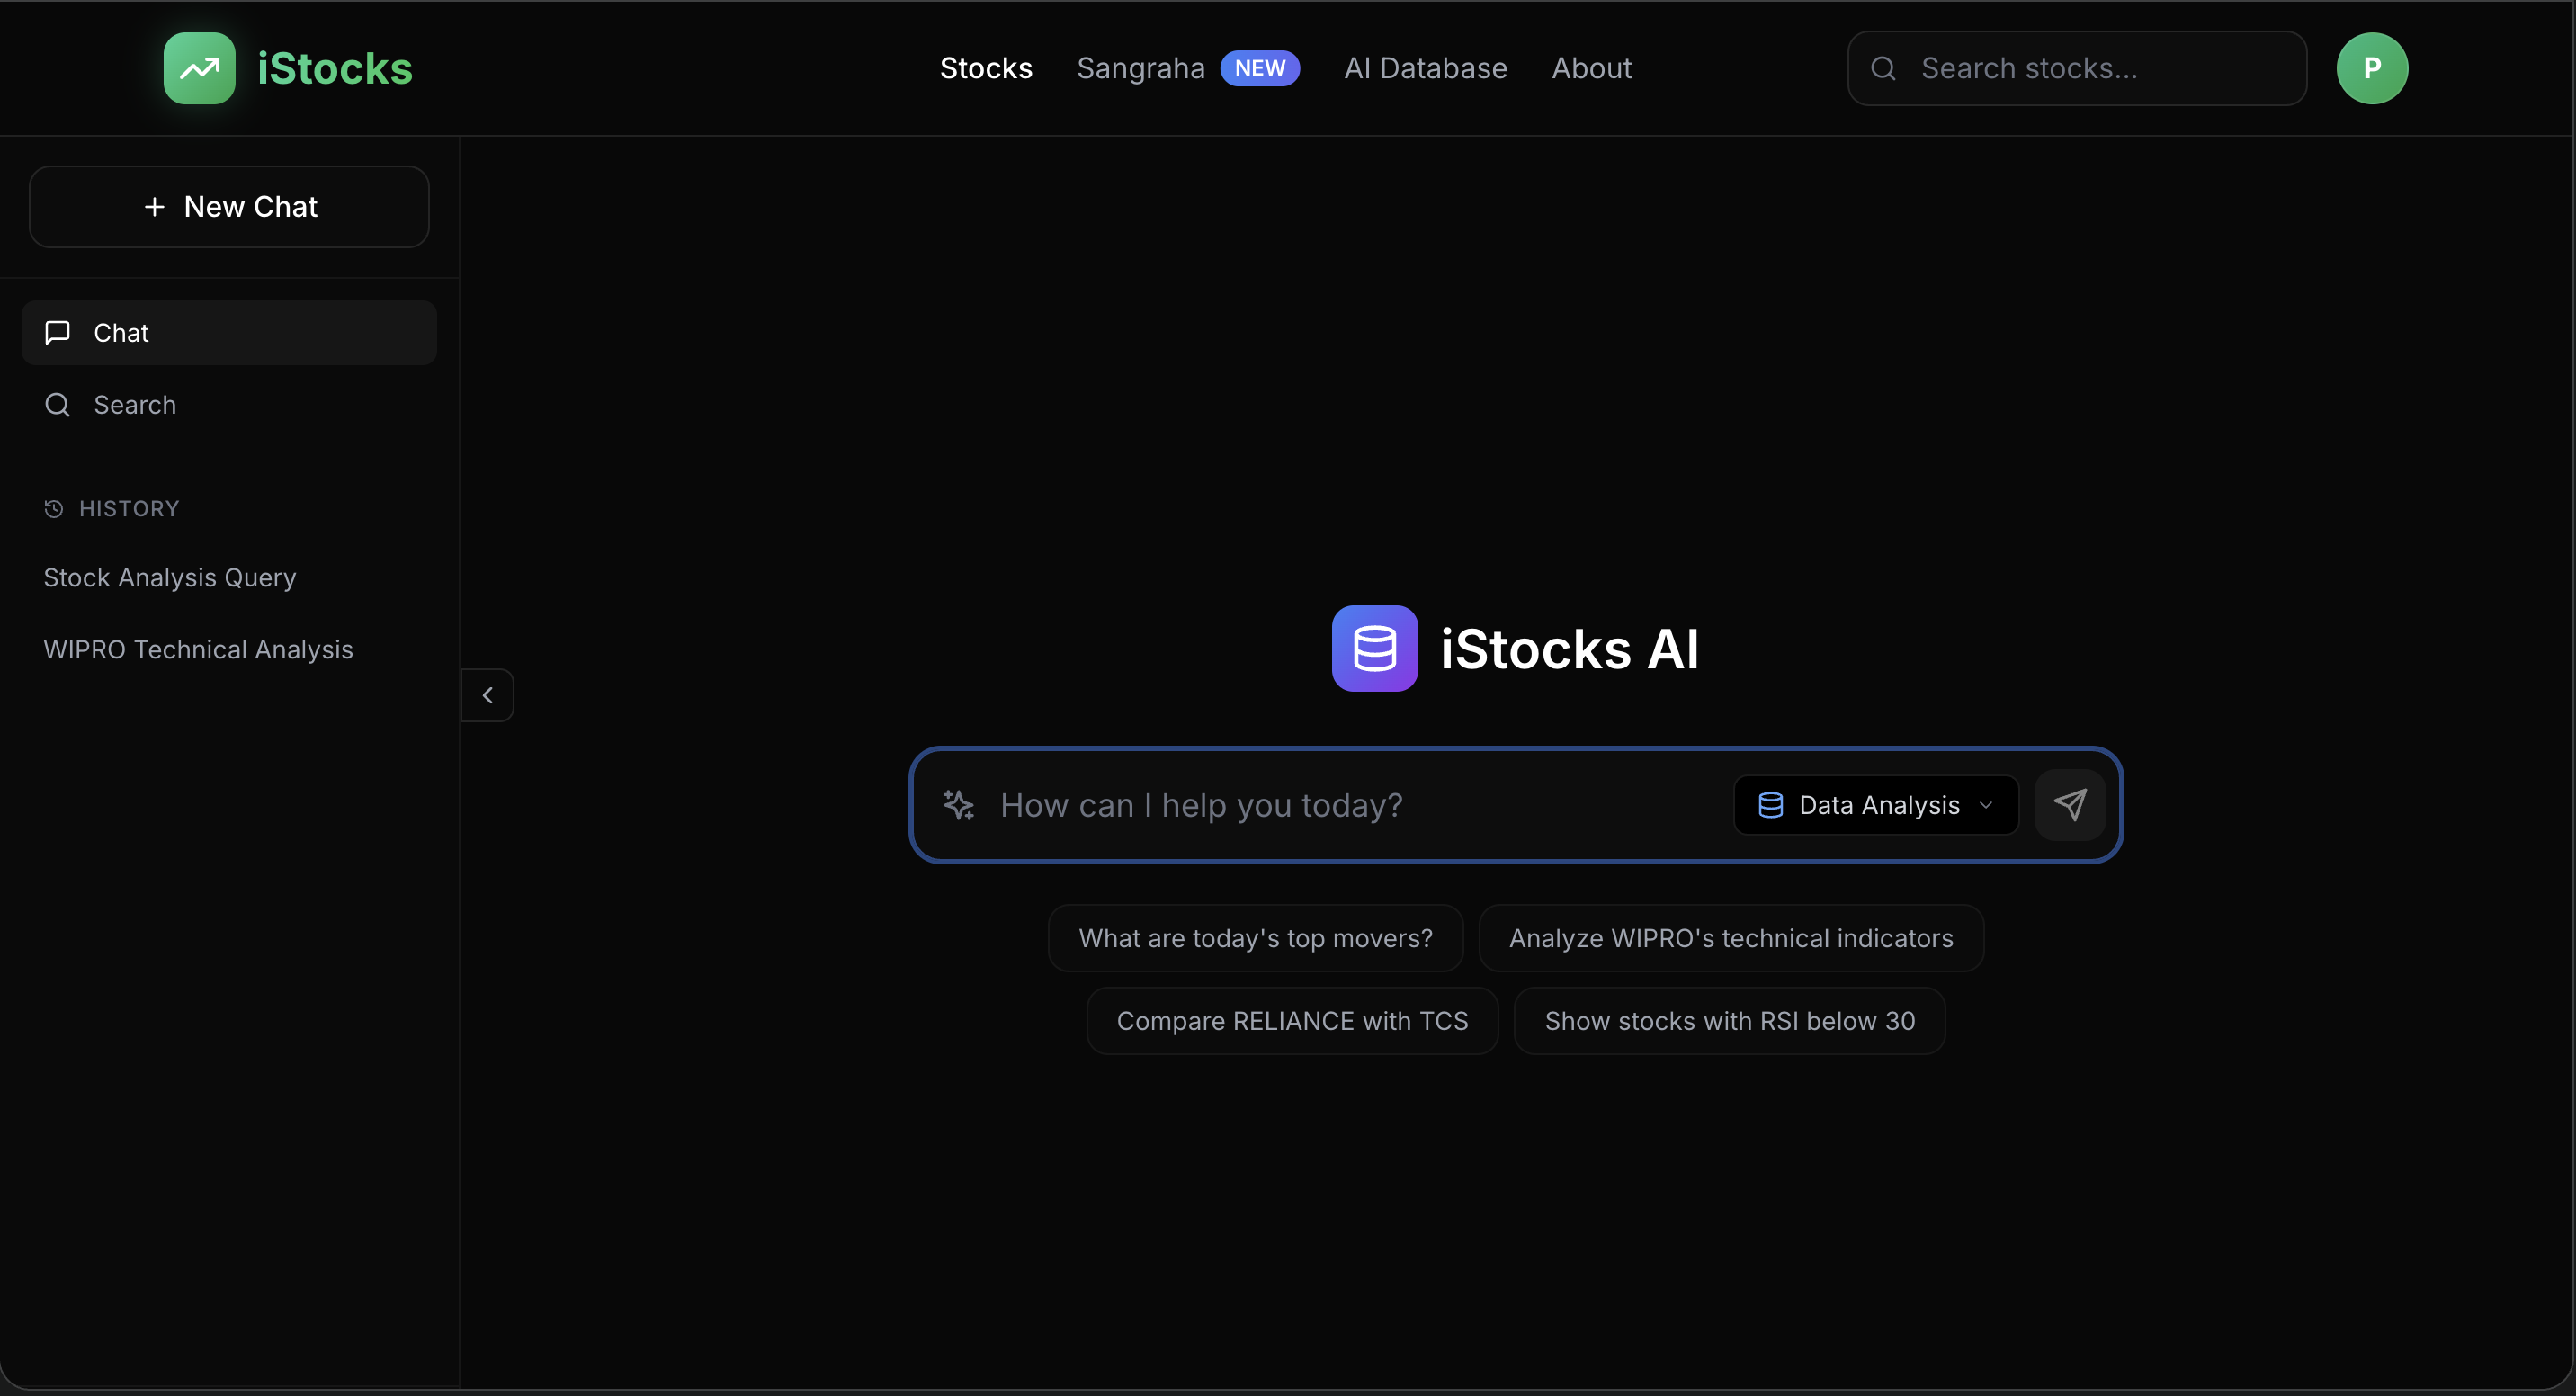
\includegraphics[width=0.95\textwidth]{Database_analysis.png}}
\end{center}

\newpage


%==============================================================================
% 2. TAM - TOTAL ADDRESSABLE MARKET
%==============================================================================
\section{Total Addressable Market (TAM)}

\subsection{Market Opportunity}

India's retail investment landscape is at an \textbf{inflection point}, creating a once-in-a-generation opportunity:

\begin{center}
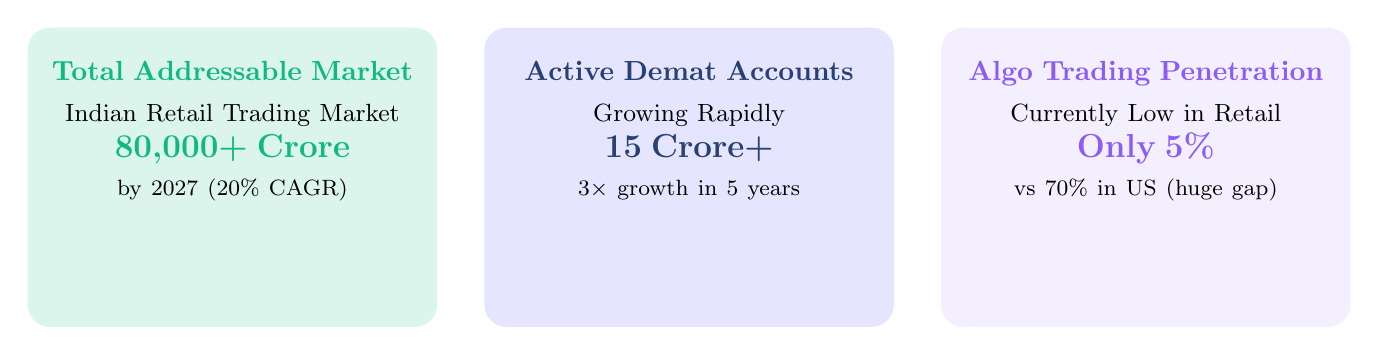
\begin{tikzpicture}
% TAM Box
\fill[primary!15, rounded corners=8pt] (0,0) rectangle (5.2,-3.8);
\node[anchor=north, text width=4.8cm, align=center] at (2.6,-0.3) {
    \textcolor{primary}{\textbf{\normalsize Total Addressable Market}}\\[0.4em]
    \small Indian Retail Trading Market\\[0.2em]
    {\large\textbf{\textcolor{primary}{\rupee 80,000+ Crore}}}\\[0.2em]
    \footnotesize by 2027 (20\% CAGR)
};

% SAM Box
\fill[blue!10, rounded corners=8pt] (5.8,0) rectangle (11,-3.8);
\node[anchor=north, text width=4.8cm, align=center] at (8.4,-0.3) {
    \textcolor{headerblue}{\textbf{\normalsize Active Demat Accounts}}\\[0.4em]
    \small Growing Rapidly\\[0.2em]
    {\large\textbf{\textcolor{headerblue}{15 Crore+}}}\\[0.2em]
    \footnotesize 3$\times$ growth in 5 years
};

% SOM Box
\fill[purpleaccent!10, rounded corners=8pt] (11.6,0) rectangle (16.8,-3.8);
\node[anchor=north, text width=4.8cm, align=center] at (14.2,-0.3) {
    \textcolor{purpleaccent}{\textbf{\normalsize Algo Trading Penetration}}\\[0.4em]
    \small Currently Low in Retail\\[0.2em]
    {\large\textbf{\textcolor{purpleaccent}{Only 5\%}}}\\[0.2em]
    \footnotesize vs 70\% in US (huge gap)
};
\end{tikzpicture}
\end{center}

\subsection{Market Size Breakdown}

\begin{statbox}
\begin{tabularx}{\textwidth}{>{\bfseries}lXr}
\toprule
\textbf{Metric} & \textbf{Details} & \textbf{Value} \\
\midrule
TAM & Indian retail trading market (equity, derivatives, MF) & \textcolor{primary}{\textbf{\rupee 80,000+ Cr}} \\
SAM & Tech-savvy active traders open to AI \& algo tools & \textcolor{headerblue}{\textbf{\rupee 12,000+ Cr}} \\
SOM & Early adopters, first 500K users in Year 1 & \textcolor{purpleaccent}{\textbf{\rupee 500+ Cr}} \\
\addlinespace
India Algo Trading Market (2025) & Institutional + Retail algo trading & \textcolor{primary}{\textbf{USD 615M}} \\
Projected Market (2030) & Growing at 25\%+ CAGR & \textcolor{primary}{\textbf{USD 2.3 Billion}} \\
Demat Accounts & Total accounts in India (2025) & \textcolor{primary}{\textbf{15 Crore+}} \\
Retail Algo Penetration & India vs US benchmark & \textcolor{accent}{\textbf{5\% vs 70\%}} \\
\bottomrule
\end{tabularx}
\end{statbox}

\subsection{Whom Are We Building For?}

\textbf{Target audience:} The next \textbf{100M+ Indian investors} who are:

\begin{multicols}{2}
\begin{itemize}[leftmargin=*]
    \item \textbf{Young (18 to 35):} Post-COVID wave of first-time investors. Comfortable with mobile apps and AI.
    \item \textbf{Tier 2/3 Cities:} 750M+ smartphone users beyond metros. Untapped, hungry for financial tools.
    \item \textbf{Regional Language Speakers:} 90\% of Indians prefer content in their local language. No trading platform serves them.
    \item \textbf{New Investors ($<$2 years):} 50\% of demat holders are new. They need guidance, not complexity.
\end{itemize}
\end{multicols}

\begin{highlightbox}[User Personas]
\begin{tabularx}{\textwidth}{>{\bfseries}p{3.5cm}X}
\faUser~Anshuman, 26 & Part-time trader. Never tried algo trading because it required coding, building infra, and it is extremely tough. Wants a no-code solution. \\
\addlinespace
\faUser~Huda, 22 & Working at HPCL. She doesn't have the time to watch charts and find the exact moment to trade at the exact time. Needs automation. \\
\addlinespace
\faUser~Nikhlesh, 22 & Working at Petronet. Understands the market well but doesn't know how to automate the process with very low latency and execute trades automatically even during his working hours. \\
\addlinespace
\faUser~Chetan, 24 & Working at a quant firm. His opinion: ``Making this platform will be very helpful for retail traders. Right now backtesting ideas is so tough, but after this they can literally give a fight.'' \\
\end{tabularx}
\end{highlightbox}

\subsection{Why Now? Market Tailwinds}

\begin{enumerate}[leftmargin=*]
    \item \textbf{Retail Trading Boom:} 15 Cr+ demat accounts, 3$\times$ growth in 5 years, young mobile-first audience.
    \item \textbf{SEBI Algo Regulation (Oct 2025):} New framework legitimized retail algo trading, moved from grey area to regulated activity.
    \item \textbf{AI Inflection Point:} LLMs and AI agents make conversational finance analysis possible for the first time.
    \item \textbf{Regional Language Gap:} 90\% of Indians prefer local language. Zero trading platforms offer NLP in regional languages.
    \item \textbf{Low Penetration:} Algo trading is only 5\% of Indian retail vs 70\% in US. Massive room to grow.
\end{enumerate}

\newpage

%==============================================================================
% 3. EASE OF PRODUCT ADOPTION
%==============================================================================
\section{Ease of Product Adoption}

\textbf{Will 100M+ Indians actually adopt this product?} Yes, and here's why:

\subsection{Zero Learning Curve}

\begin{featurebox}[Conversational AI = Universal Interface]
\textbf{The chat interface is the product.} Every Indian who uses WhatsApp already knows how to use iStocks. Just type a question, ``How is Reliance doing?'', and get a professional analysis. No charts to learn, no buttons to find, no jargon to decode.
\end{featurebox}

\subsection{Five Pillars of Adoptability}

\begin{tabularx}{\textwidth}{>{\centering\arraybackslash}p{1cm}>{\bfseries}p{3.5cm}X}
\toprule
& \textbf{Pillar} & \textbf{Why It Drives Adoption} \\
\midrule
\faComments & Conversational AI & No learning curve. Like texting a stock expert friend. Ask in plain language, get analysis in seconds. \\
\addlinespace
\faGlobe & Regional Languages & Hindi, Tamil, Telugu, Marathi \& more. First platform to serve Bharat, not just India's English-speaking 10\%. \\
\addlinespace
\faHandHoldingUsd & Free to Start & Zero cost barrier. Freemium model lets anyone try before committing. No credit card needed. \\
\addlinespace
\faMobile & Web + Android & Available at istocks.codes and as Android APK. Will soon be on Play Store. Share via WhatsApp link. Works on low-end phones. \\
\addlinespace
\faClock & Speed to Value & Under 30 seconds from first visit to first AI insight. No signup needed for basic analysis. \\
\bottomrule
\end{tabularx}

\begin{center}
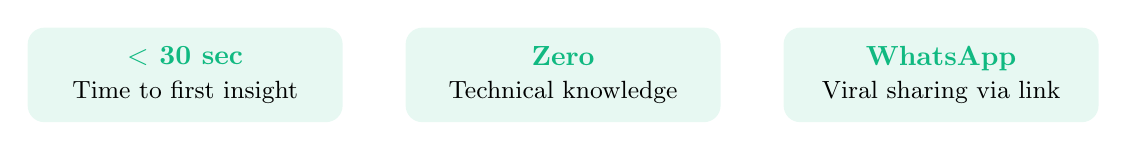
\begin{tikzpicture}
\fill[primary!10, rounded corners=6pt] (0,0) rectangle (4,-1.2);
\node[align=center] at (2,-0.6) {\textbf{\textcolor{primary}{{$<$ 30 sec}}}\\\small Time to first insight};

\fill[primary!10, rounded corners=6pt] (4.8,0) rectangle (8.8,-1.2);
\node[align=center] at (6.8,-0.6) {\textbf{\textcolor{primary}{Zero}}\\\small Technical knowledge};

\fill[primary!10, rounded corners=6pt] (9.6,0) rectangle (13.6,-1.2);
\node[align=center] at (11.6,-0.6) {\textbf{\textcolor{primary}{WhatsApp}}\\\small Viral sharing via link};
\end{tikzpicture}
\end{center}

\newpage

%==============================================================================
% 4. MONETIZATION
%==============================================================================
\section{Power User Monetization}

\subsection{Revenue Model}

iStocks has a \textbf{two-phase revenue strategy} designed for sustainable, scalable growth:

\begin{highlightbox}[Revenue Stream 1: Subscription Plans (Immediate)]
This is our \textbf{primary revenue driver from Day 1}. Users pay for premium AI features, advanced analysis, and algo deployment.

\begin{tabularx}{\textwidth}{>{\bfseries}p{2.5cm}p{3.5cm}X}
\toprule
\textbf{Tier} & \textbf{Price} & \textbf{Includes} \\
\midrule
Free & \rupee0/month & Basic AI chat (limited queries), 5 stock dashboards, community access \\
\addlinespace
Pro & \rupee299/month & Unlimited AI queries, 40+ indicators, priority response, Sangraha access \\
\addlinespace
Elite & \rupee999/month & Algo deployment, backtesting, expert network, API access, premium strategies \\
\bottomrule
\end{tabularx}
\end{highlightbox}

\begin{highlightbox}[Revenue Stream 2: Becoming a Broker (Year 1+)]
Right now, we will earn only through subscriptions. However, after one year of building trust, user base, and regulatory compliance, \textbf{iStocks will become a registered broker}. This will unlock brokerage commissions on every trade executed through our platform.\\[0.5em]
\textbf{Why this matters:} Brokerage revenue at scale is the \textbf{largest revenue driver} in the Indian fintech space. Zerodha (\rupee8,320 Cr), Angel One (\rupee4,275 Cr), and Groww (\rupee3,145 Cr) all earn the majority of their revenue from brokerage. By becoming a broker, iStocks transitions from a SaaS tool to a \textbf{full-stack financial platform} with compounding revenue.\\[0.5em]
\textbf{Industry Standard:} \rupee20 per executed order or 0.03\% of turnover.
\end{highlightbox}

\begin{highlightbox}[Revenue Stream 3: Strategy Marketplace]
Premium strategies on Sangraha where creators earn and the platform takes a \textbf{15 to 20\% cut}.\\[0.3em]
Expert Network: Verified traders manage portfolios for followers via a \textbf{profit-sharing model}.
\end{highlightbox}

\newpage

%==============================================================================
% 5. COMPETITIVE LANDSCAPE & MOAT
%==============================================================================
\section{Moat: Why iStocks Will Win}

\subsection{Competitive Landscape}

\begin{center}
\small
\renewcommand{\arraystretch}{1.4}
\begin{tabularx}{\textwidth}{p{2.8cm}ccccccc}
\toprule
\rowcolor{primary!15}
\textbf{Feature} & \textbf{Zerodha} & \textbf{Groww} & \textbf{Angel One} & \textbf{TradingView} & \textbf{Streak} & \cellcolor{primary!30}\textbf{iStocks} \\
\midrule
AI Chatbot & \textcolor{accent}{\ding{55}} & \textcolor{accent}{\ding{55}} & \textcolor{accent}{\ding{55}} & \textcolor{accent}{\ding{55}} & \textcolor{accent}{\ding{55}} & \textcolor{primary}{\ding{51}} \\
Regional NLP & \textcolor{accent}{\ding{55}} & \textcolor{accent}{\ding{55}} & \textcolor{accent}{\ding{55}} & \textcolor{accent}{\ding{55}} & \textcolor{accent}{\ding{55}} & \textcolor{primary}{\ding{51}} \\
No-Code Bots & \textcolor{accent}{\ding{55}} & \textcolor{accent}{\ding{55}} & \textcolor{accent}{\ding{55}} & \textcolor{accent}{\ding{55}} & Partial & \textcolor{primary}{\ding{51}} \\
Strategy Repo & \textcolor{accent}{\ding{55}} & \textcolor{accent}{\ding{55}} & \textcolor{accent}{\ding{55}} & Ideas & Partial & \textcolor{primary}{\ding{51}} \\
Trading Agent & \textcolor{accent}{\ding{55}} & \textcolor{accent}{\ding{55}} & \textcolor{accent}{\ding{55}} & \textcolor{accent}{\ding{55}} & \textcolor{accent}{\ding{55}} & \textcolor{primary}{\ding{51}} \\
40+ Indicators & Kite & \textcolor{accent}{\ding{55}} & Basic & \textcolor{primary}{\ding{51}} & Basic & \textcolor{primary}{\ding{51}} \\
\midrule
Revenue (FY24) & \rupee8,320 Cr & \rupee3,145 Cr & \rupee4,275 Cr & \$250M & \rupee50 Cr & Pre-Rev \\
\bottomrule
\end{tabularx}
\end{center}

\textbf{Key Insight:} No existing player combines \textbf{NLP + AI agents + regional languages + strategy marketplace}. We are creating a new category.

\subsection{Five Pillars of Defensibility}

\begin{purplebox}[Our Moat is a Compounding Advantage]
\begin{enumerate}[leftmargin=*]
    \item \textbf{First Mover in NLP Trading:} No Indian platform combines NLP + AI trading agents + regional language support. We define the category and set the standard.
    
    \item \textbf{Data Network Effects:} Every user query makes our AI smarter. More users = better recommendations = more users. Classic flywheel effect that becomes harder to replicate over time.
    
    \item \textbf{Community Strategy Repository (Sangraha):} User-generated strategies create content lock-in. Fork, backtest, deploy, like GitHub for trading. This grows organically and is nearly impossible to replicate.
    
    \item \textbf{Regional Language Lock-in:} 90\% of India doesn't use English daily. Once a user experiences intelligent stock analysis in Hindi or Tamil, switching to an English-only platform is painful.
    
    \item \textbf{AI Agent Ecosystem:} Expert Network + Bot Marketplace creates two-sided marketplace dynamics. Experts earn by sharing strategies, users profit by following them. \textit{Everyone stays}.
\end{enumerate}
\end{purplebox}

\newpage

%==============================================================================
% 6. RISKS & MITIGATION
%==============================================================================
\section{What Could Cause Failure and Mitigation}

\subsection{Risk Analysis}

\begin{riskbox}[Risk 1: Execution Risk]
\textbf{Threat:} Not iterating fast enough, losing momentum against well-funded incumbents like Zerodha or Groww.\\[0.3em]
\begin{fixbox}
\textcolor{primary}{\textbf{Mitigation:}} Relentless execution cadence. Ship weekly. Stay lean and founder-led. \textbf{Hard work is the only answer}, and the founding team is committed to outworking everyone.
\end{fixbox}
\end{riskbox}

\begin{riskbox}[Risk 2: Regulatory Risk]
\textbf{Threat:} SEBI tightens algo trading rules or bans retail algo APIs.\\[0.3em]
\begin{fixbox}
\textcolor{primary}{\textbf{Mitigation:}} Compliance-first approach from Day 1. Partner exclusively with SEBI-registered brokers. Stay within regulatory sandbox. The Oct 2025 SEBI framework actually \textit{legitimized} retail algo trading.
\end{fixbox}
\end{riskbox}

\begin{riskbox}[Risk 3: Big Player Entry]
\textbf{Threat:} Zerodha or Groww launches their own AI chatbot feature.\\[0.3em]
\begin{fixbox}
\textcolor{primary}{\textbf{Mitigation:}} Speed of innovation is our weapon. NLP in regional languages + community strategy repo + AI agent ecosystem is a \textit{platform}, not a feature. Hard to replicate quickly. First-mover data advantage compounds.
\end{fixbox}
\end{riskbox}

\begin{riskbox}[Risk 4: AI Hallucination / Trust]
\textbf{Threat:} AI gives incorrect stock advice leading to user losses and trust erosion.\\[0.3em]
\begin{fixbox}
\textcolor{primary}{\textbf{Mitigation:}} Ground AI in real data: 40+ technical indicators, live prices, historical trends. RAG pipeline with verified data sources. Mandatory disclaimers. Transparency via ``show me the data'' feature.
\end{fixbox}
\end{riskbox}

\begin{riskbox}[Risk 5: Market Downturn]
\textbf{Threat:} Bear market reduces retail trading volumes and user interest.\\[0.3em]
\begin{fixbox}
\textcolor{primary}{\textbf{Mitigation:}} Expand product beyond equities to mutual funds, FDs, gold, and government bonds, covering \textbf{short-term and intermediate-term investments}. iStocks becomes a comprehensive wealth platform, not just a stock tool.
\end{fixbox}
\end{riskbox}

\newpage

%==============================================================================
% 7. REFERENCES
%==============================================================================
\section{References and Sources}

\begin{enumerate}[leftmargin=*]
    \item \textbf{SEBI Annual Report 2024-25}: Demat account growth statistics, retail investor participation, algo trading regulatory framework (effective Oct 2025).
    
    \item \textbf{IMARC Group Research (2025)}: India Algorithmic Trading Market valued at USD 615.61M in 2025, projected to reach USD 2.3B by 2030.\\
    \url{https://www.imarcgroup.com}
    
    \item \textbf{Grand View Research}: Global and India algorithmic trading market size, growth trends, and competitive segment analysis.\\
    \url{https://www.grandviewresearch.com}
    
    \item \textbf{NSE / BSE Official Data}: Real-time and historical stock data. Active demat accounts crossed 15 Crore in 2025.
    
    \item \textbf{KPMG India Fintech Report 2024}: Retail investment trends, digital adoption in Tier 2/3 cities, regional language preferences.\\
    \url{https://kpmg.com/in}
    
    \item \textbf{Zerodha, Groww, Angel One Annual Reports (FY24)}: Revenue benchmarks (\rupee8,320 Cr, \rupee3,145 Cr, \rupee4,275 Cr), user growth, and feature gaps used for competitive analysis.
    
    \item \textbf{Google India Language Diversity Report}: 90\% of Indian internet users prefer regional language content; identifies massive unserved gap in financial services.
    
    \item \textbf{Republic World / ScanX Trade / QuantInsti (2025)}: Algo trading penetration analysis: 67\% in F\&O derivatives, only 5\% in retail equity cash segment.\\
    \url{https://scanx.trade} ~|~ \url{https://quantinsti.com}
    
    \item \textbf{Fintrens / WelthWest (2025)}: SEBI algorithmic trading framework analysis and its impact on retail trader accessibility.
    
    \item \textbf{iStocks Platform Documentation}: Feature specifications and product documentation.\\
    \url{https://istocks.codes}
\end{enumerate}

\vspace{2cm}

% ========== CLOSING ==========
\begin{center}
\rule{0.4\textwidth}{0.5pt}
\end{center}

\vfill

\begin{center}
    \textcolor{primary}{\Large\faChartLine}\\[0.5cm]
    {\large\textbf{iStocks}}\\[0.2cm]
    {\small AI-Native Investment Platform for Bharat}\\[0.3cm]
    {\small Empowering Every Indian to Invest Smarter, In Their Own Language}\\[1cm]
    
    \textcolor{textgray}{\small Live: \url{https://istocks.codes}}
\end{center}

\vspace{2cm}

\begin{flushright}
    \textbf{CREATED BY: Priyanshu}
\end{flushright}

\end{document}
